%
% Copyright 2021 Joel Feldman, Andrew Rechnitzer and Elyse Yeager.
% This work is licensed under a Creative Commons Attribution-NonCommercial-ShareAlike 4.0 International License.
% https://creativecommons.org/licenses/by-nc-sa/4.0/
%
\graphicspath{{figures/rootFinding/}}
%\renewcommand{\theequation}{\thechapter.\arabic{equation}}
%\renewcommand{\thetheorem}{\thechapter.\arabic{theorem}}
%\renewcommand{\thebc}{\thechapter.\arabic{theorem}}
%\renewcommand{\theeg}{\thechapter.\arabic{theorem}}

\chapter{Root Finding}\label{app root finding}

To this point you have found solutions to equations almost
exclusively by algebraic manipulation. This is possible only
for the artificially simple equations of problem sets and
tests. In the ``real world'' it is very common to encounter
equations that cannot be solved by algebraic manipulation.
For example, you found, by completing a square, that the 
solutions to the quadratic equation $ax^2+bx+c=0$ are 
$x=\big(-b\pm\sqrt{b^2-4ac}\big)/2a$.
But it is known that there simply does not exist a corresponding formula
for the roots of a general polynomial of degree five or more.
Fortunately, encountering such an equation is not the end of the
world, because usually one does not need to know the solutions
exactly. One only needs to know them to within some specified 
degree of accuracy. For example, one rarely needs to know $\pi$ 
to more than a few decimal places. There is a whole subject, 
called numerical analysis, that concerns using algorithms to solve 
equations (and perform other tasks) approximately, to any desired 
degree of accuracy. 

We have already had, in Examples \ref{eg pre bisection} and \ref{eg bisection},
and the lead up to them, a really quick introduction to the bisection method, 
which is a crude, but effective, algorithm for finding approximate solutions to equations 
of the form $f(x)=0$. We shall shortly use a little calculus
to derive a very efficient algorithm for finding approximate solutions
to such equations. But first here is a simple
example which provides a review of some of the basic ideas of root
finding and the bisection method.

\begin{eg}\label{eg:rootFindingA}
Suppose that we are given some function $f(x)$ and we have to find
solutions to the equation $f(x)=0$. To be concrete, suppose
that $f(x) = 8x^3+12x^2+6x-15$. How do we go about solving
$f(x)=0$? To get a rough idea of the lay of the land, sketch
the graph of $f(x)$. First observe that
\begin{itemize}\itemsep1pt \parskip0pt \parsep0pt
\item when $x$ is very large and negative, $f(x)$ is very large 
and negative
\item when $x$ is very large and positive, $f(x)$ is very large 
and positive 
\item when $x=0$, $f(x) =f(0) = -15<0$
\item when $x=1$, $f(x) =f(1) = 11>0$
\item $f'(x) = 24x^2+24x+6 = 24\big(x^2+x+\frac{1}{4}\big)
          =24\big(x+\frac{1}{2}\big)^2\ge 0$ for all $x$.
      So $f(x)$ increases monotonically with $x$. The graph has
      a tangent of slope $0$ at $x=-\frac{1}{2}$ and tangents of
      strictly positive slope everywhere else.
\end{itemize}
This tells us that the graph of $f(x)$ looks like
\begin{efig}
\begin{center}
   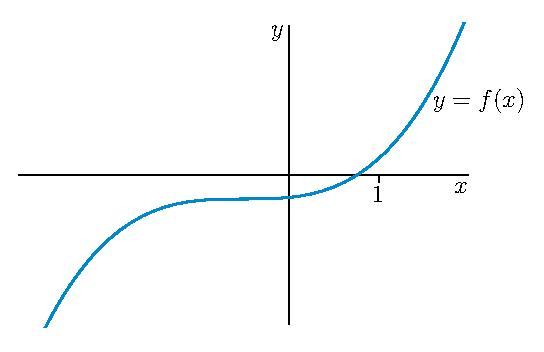
\includegraphics{rootFindingCubic}
\end{center}
\end{efig}
Since $f(x)$ strictly increases\footnote{By ``$f(x)$ is strictly increasing'' 
we mean that $f(a)<f(b)$ whenever $a<b$. 
As $f'(x)>0$ for all $x\ne-\frac{1}{2}$, $f(x)$ is strictly increasing even 
as $x$ passes through $-\frac{1}{2}$. For example, for any $x>-\frac{1}{2}$, 
the mean value theorem (Theorem~\ref{thm:DIFFmvt}), tells us that there is 
a $c$ strictly between $-\frac{1}{2}$ and $x$ such that
$f(x)-f\big(-\frac{1}{2}\big) = f'(c)\big(x+\frac{1}{2}\big)>0$.} as 
$x$ increases, $f(x)$ can take the value zero for at most one value of $x$.
\begin{itemize}\itemsep1pt \parskip0pt \parsep0pt
\item
Since $f(0)<0$ and $f(1)>0$ and $f$ is continuous, $f(x)$ must
pass through $0$ as $x$ travels from $x=0$ to $x=1$, by Theorem 
\ref{thm ivt} (the intermediate value theorem). So $f(x)$ takes the value zero 
for some $x$ between $0$ and $1$. We will often write this as  ``the root is 
$x=0.5\pm 0.5$'' to indicate the uncertainty. 
\item 
To get closer to the root, we evaluate $f(x)$ halfway between $0$ and $1$.
\begin{equation*}
f\big(\tfrac{1}{2}\big) = 8\big(\tfrac{1}{2}\big)^3+12\big(\tfrac{1}{2}\big)^2
                             +6\big(\tfrac{1}{2}\big)-15
                        = -8
\end{equation*}
Since $f\big(\frac{1}{2}\big)<0$ and $f(1)>0$ and $f$ is continuous, 
$f(x)$ must take the value zero for some $x$ 
between $\frac{1}{2}$ and $1$. The root is $0.75\pm 0.25$.

\item 
To get still closer to the root, we evaluate $f(x)$ halfway between 
$\frac{1}{2}$ and $1$.
\begin{equation*}
f\big(\tfrac{3}{4}\big) = 8\big(\tfrac{3}{4}\big)^3+12\big(\tfrac{3}{4}\big)^2
                             +6\big(\tfrac{3}{4}\big)-15
                        = -\tfrac{3}{8}
\end{equation*}
Since $f\big(\frac{3}{4}\big)<0$ and $f(1)>0$ and $f$ is continuous, 
$f(x)$ must take the value zero for some $x$ 
between $\frac{3}{4}$ and $1$. The root is $0.875\pm 0.125$.
\item And so on.
\end{itemize}
\end{eg}

The root finding strategy used in Example \ref{eg:rootFindingA} is 
called the bisection method. The bisection method will home in on a root of the
function $f(x)$ whenever
\begin{itemize}
\item
$f(x)$ is continuous ($f(x)$ need not have a derivative) and
\item
you can find two numbers $a_1<b_1$ with $f(a_1)$ and $f(b_1)$ being of opposite 
sign. 
\end{itemize}
Denote by $I_1$ the interval $[a_1,b_1]=\big\{x\ \big|\ a_1\le x\le b_1\big\}$.
Once you have found the interval $I_1$, the bisection method generates a sequence $I_1$, 
         $I_2$, 
         $I_3$, $\cdots$ 
of intervals by the following rule.
\begin{impeqn}[bisection method]\label{eq:APPbisection}
Denote by $c_n=\frac{a_n+b_n}{2}$ the midpoint of the interval $I_n=[a_n,b_n]$. 
If $f(c_n)$ has the same sign as $f(a_n)$, then
  \begin{equation*}
    I_{n+1}=[a_{n+1},b_{n+1}]\quad\text{with}\quad
               a_{n+1}=c_n,\  b_{n+1}=b_n
  \end{equation*}
and if 
$f(c_n)$ and $f(a_n)$ have opposite signs, then
  \begin{equation*}
    I_{n+1}=[a_{n+1},b_{n+1}]\quad\text{with}\quad
             a_{n+1}=a_n,\  b_{n+1}=c_n
  \end{equation*}
\end{impeqn}
This rule was chosen so that $f(a_n)$ and $f(b_n)$ have opposite sign for 
every $n$.
Since $f(x)$ is continuous, $f(x)$ has a zero in each interval $I_n$.
Thus each step reduces the error bars by a factor of $2$. That isn't too 
bad, but we can come up with something that is much more efficient. 
We just need a little calculus.

%%%%%%%%%%%%%%%%%%%%%%%%%%%%%%%%%%%%%%%%%%%%%%%%%%%%%%%%%%%%%%%
\section{Newton's Method}\label{sec_C_1}
%%%%%%%%%%%%%%%%%%%%%%%%%%%%%%%%%%%%%%%%%%%%%%%%%%%%%%%%%%%%%%%%
Newton's method\footnote{The algorithm that we are about to describe grew out of a method that Newton wrote about in 1669. But the modern method incorporates
substantial changes introduced by Raphson in 1690 and Simpson in 1740.},  
also known as the Newton-Raphson method, is another technique for generating 
numerical approximate solutions to equations of the form $f(x)=0$. For 
example, one can easily get a good approximation to $\sqrt{2}$ by 
applying Newton's method to the equation $x^2-2=0$. This will be done in 
Example \ref{eg:NTMsqrttwo}, below.

Here is the derivation of Newton's method. We start by simply making a
guess for the solution. For example, we could base the guess on a sketch
of the graph of $f(x)$. Call the initial guess $x_1$. 
Next recall, from Theorem \ref{thm:DIFFtangentLine}, that the tangent 
line to $y=f(x)$ at $x=x_1$ is $y=F(x)$, where
\begin{equation*}
F(x) = f(x_1) + f'(x_1)\,(x-x_1)
\end{equation*}
Usually $F(x)$ is a pretty good approximation to $f(x)$ for $x$ near $x_1$. 
So, instead of trying to solve $f(x)=0$, we solve the linear equation
$F(x)=0$ and call the solution $x_2$.
\begin{align*}
0=F(x)=f(x_1) + f'(x_1)\,(x-x_1)
&\iff x-x_1=-\frac{f(x_1)}{f'(x_1)} \\
&\iff x= x_2= x_1 -\frac{f(x_1)}{f'(x_1)}
\end{align*}
Note that if $f(x)$ were a linear function, then $F(x)$ would be exactly $f(x)$
and $x_2$ would solve $f(x)=0$ exactly.
\begin{efig}
\begin{center}
   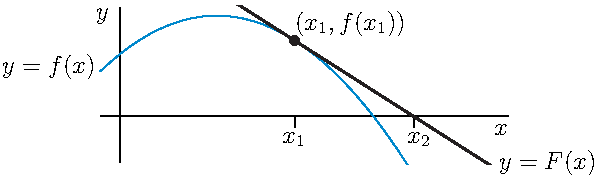
\includegraphics{NewtonM}
\end{center}
\end{efig}

Now we repeat, but starting with the (second) guess $x_2$ rather than $x_1$.
This gives the (third) guess $x_3= x_2 -\frac{f(x_2)}{f'(x_2)}$. And so
on. By way of summary, Newton's method is
\begin{enumerate}
\item Make a preliminary guess $x_1$.
\item Define $x_2=x_1-\frac{f(x_1)}{f'(x_1)}$.
\item Iterate. That is, for each natural number $n$,
    once you have computed $x_n$, define 
   \begin{impeqn}[Newton's method]\label{eq:APPnewton}
  \begin{equation*}
    x_{n+1}=x_n-\frac{f(x_n)}{f'(x_n)}
  \end{equation*}
  \end{impeqn}
\end{enumerate}

\begin{eg}[Approximating $\sqrt{2}$]\label{eg:NTMsqrttwo}
In this example we compute, approximately, the square root of two.
We will of course pretend that we do not already know that
$\sqrt{2}=1.41421\cdots$. So we cannot find it by solving, approximately, 
the equation $f(x)=x-\sqrt{2}=0$. Instead we apply Newton's method to 
the equation
\begin{equation*}
f(x)=x^2-2=0
\end{equation*}
Since $f'(x)=2x$, Newton's method says that we should generate
approximate solutions by iteratively applying
\begin{equation*}
x_{n+1}=x_n-\frac{f(x_n)}{f'(x_n)}=x_n-\frac{x_n^2-2}{2x_n}
=\frac{x_n}{2} +\frac{1}{x_n}
\end{equation*}
We need a starting point.
Since $1^2=1<2$ and $2^2=4>2$, the square root of two must be between $1$
and $2$, so let's start Newton's method with the initial guess $x_1=1.5$.
Here goes\footnote{The following computations have been carried out in double precision, which is computer speak for about 15 significant digits. We are displaying each $x_n$ rounded to 10 significant digits (9 decimal places).
So each displayed $x_n$ has not been impacted by roundoff error, and still 
contains more decimal places than are usually needed.}:
\begin{align*}
x_1&=1.5\cr
x_2&=\frac{1}{2} x_1+\frac{1}{x_1}
=\frac{1}{2}(1.5)+\frac{1}{1.5}\\
&=1.416666667  \displaybreak[0] \\ 
x_3&=\frac{1}{2} x_2+\frac{1}{x_2}
=\frac{1}{2}(1.416666667)+\frac{1}{1.416666667} \\ 
&=1.414215686  \displaybreak[0] \\ 
x_4&=\frac{1}{2} x_3+\frac{1}{x_3}
=\frac{1}{2}(1.414215686)+\frac{1}{1.414215686} \\ 
&=1.414213562  \displaybreak[0] \\ 
x_5&=\frac{1}{2} x_4+\frac{1}{x_4}
=\frac{1}{2}(1.414213562)+\frac{1}{1.414213562}\\
&=1.414213562
\end{align*}
It looks like the $x_n$'s, rounded to nine decimal places, have stabilized
to $1.414213562$. So it is reasonable to guess that $\sqrt{2}$, rounded
to nine decimal places, is exactly $1.414213562$. Recalling that all numbers
$1.4142135615 \le y < 1.4142135625$ round to $1.414213562$, we can
check our guess by evaluating $f(1.4142135615)$ and $f(1.4142135625)$.
Since  $f(1.4142135615)=-2.5\times 10^{-9}<0$ and
                  $f(1.4142135625)=3.6\times 10^{-10}>0$
the square root of two must indeed be between $1.4142135615$ and
$1.4142135625$.

\end{eg}

\begin{eg}[Approximating $\pi$]\label{eg:exNTMpi}
In this example we compute, approximately, $\pi$ by
applying Newton's method to the equation
\begin{equation*}
f(x)=\sin x=0
\end{equation*}
starting with $x_1=3$. 
Since $f'(x)=\cos x$, Newton's method says that we should generate
approximate solutions by iteratively applying
\begin{equation*}
x_{n+1}=x_n-\frac{f(x_n)}{f'(x_n)}=x_n-\frac{\sin x_n}{\cos x_n}
=x_n-\tan x_n
\end{equation*}
Here goes
\begin{align*}
x_1&=3\\
x_2&=x_1-\tan x_1
=3-\tan 3\\
&=3.142546543\\
x_3&
=3.142546543-\tan 3.142546543\\
&=3.141592653\\
x_4&
=3.141592653-\tan 3.141592653\\
&=3.141592654\\
x_5&
=3.141592654-\tan 3.141592654\\
&=3.141592654
\end{align*}
Since  $f(3.1415926535)=9.0\times 10^{-11}>0$ and
$f(3.1415926545)=-9.1\times 10^{-11}<0$,
$\pi$ must be between $3.1415926535$ and $3.1415926545$.
Of course to compute $\pi$ in this way, we (or at least our computers) have to be able to evaluate $\tan x$ for various values of $x$. Taylor expansions can 
help us do that. See Example~\ref{eg:taylorapprox}.
\end{eg}

\begin{eg}[wild instability]\label{eg:NTMbad}
This example illustrates how Newton's method can go badly wrong if your
initial guess is not good enough. We'll try to solve the equation
\begin{equation*}
f(x)=\arctan x=0
\end{equation*}
starting with $x_1=1.5$. (Of course the solution to $f(x)=0$ is just $x=0$; 
we chose $x_1=1.5$ for demonstration purposes.) Since the derivative
$
f'(x)=\frac{1}{1+x^2}
$,
Newton's method gives
\begin{equation*}
x_{n+1}=x_n-\frac{f(x_n)}{f'(x_n)}=x_n-(1+x_n^2)\arctan x_n
\end{equation*}
So\footnote{Once again, the following computations have been carried 
out in double precision. This time, it is clear that the $x_n$'s are 
growing madly as $n$ increases.  So there is not much point to displaying 
many decimal places and we have not done so.}
\begin{align*}
x_1&=1.5\\
x_2&=1.5-(1+1.5^2)\arctan 1.5=-1.69\\
x_3&=-1.69-(1+1.69^2)\arctan (-1.69)=2.32\\
x_4&=2.32-(1+2.32^2)\arctan (2.32)=-5.11\\
x_5&=-5.11-(1+5.11^2)\arctan (-5.11)=32.3\\
x_6&=32.3-(1+32.3^2)\arctan (32.3)=-1575\\
x_7&=3,894,976
\end{align*}
Looks pretty bad! Our $x_n$'s are not settling down at all!

The figure below shows what went wrong. In this figure,
$y=F_1(x)$ is the tangent line to $y=\arctan x$ at $x=x_1$.
Under Newton's method, this tangent line crosses the $x$--axis at $x=x_2$.
Then $y=F_2(x)$ is the tangent to $y=\arctan x$ at $x=x_2$.
Under Newton's method, this tangent line crosses the $x$--axis at $x=x_3$.
And so on. 

The problem arose because the $x_n$'s were far enough from the solution, $x=0$, that the tangent line approximations,
\vadjust{
\begin{efig}
\begin{center}
   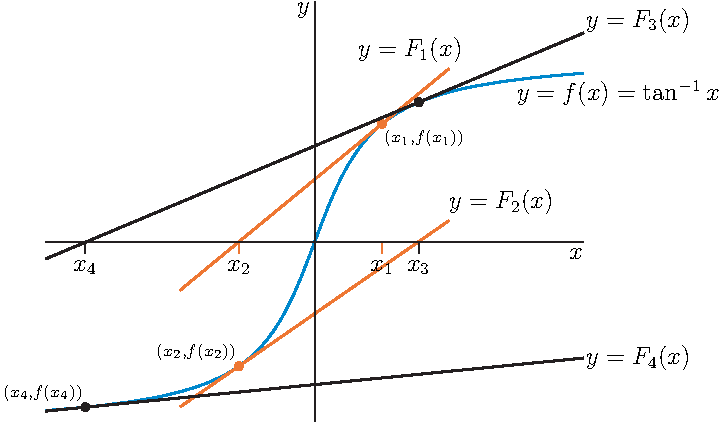
\includegraphics{badNewtonF}
\end{center}
\end{efig}
}
while good approximations to $f(x)$ for $x\approx x_n$, were very 
poor approximations to $f(x)$ for $x\approx 0$. 
In particular, $y=F_1(x)$ (i.e. the tangent line at $x=x_1$)
was a bad enough approximation to $y=\arctan x$ for $x\approx0$ that $x=x_2$ (i.e. the value of $x$ where $y=F_1(x)$ crosses the $x$-axis) is farther from the solution $x=0$ than our original guess $x=x_1$. If we had started with
$x_1=0.5$ instead of $x_1=1.5$, Newton's method would have succeeded very nicely:
\begin{align*}
x_1=0.5\qquad
x_2=-0.0796\qquad
x_3=0.000335\qquad
x_4=-2.51\times 10^{-11}
\end{align*}

\begin{comment}
We have
\begin{align*}
x_n-(1+x_n)^2\arctan x_n=-x_n
&\iff (1+x_n)^2\arctan x_n=2x_n \\
&\iff \frac{(1+x_n)^2}{2x_n}\arctan x_n=1 \\
&\iff |x_n|=1.392
\end{align*}
\end{comment}
\end{eg}

\begin{eg}[interest rate]\label{eg:NTMcar}
A car dealer sells a new car for \$23,520. He also offers to finance the same
car for payments of \$420 per month for five years. What interest rate
is this dealer charging?

\soln
By way of preparation, we'll start with a simpler problem.
Suppose that you will have to make a single \$420 payment $n$ months 
in the future. The simpler problem is to determine how much money you have 
to deposit now in an account that pays an interest rate of  $100 r\%$ per month, 
compounded monthly\footnote{``Compounded monthly'', means that, each month, interest is paid on the accumulated interest that was paid in all previous months.}, in order to be able to make the \$420 payment in $n$ months.

Let's denote by $P$ the initial deposit. Because the  interest rate is  
$100 r\%$ per month, compounded monthly,
\begin{itemize}\itemsep1pt \parskip0pt \parsep0pt
\item
the first month's interest is $P\times r$. 
So at the end of month \#1, the account balance is $P+P\,r=P(1+r)$.
\item
The second month's interest is $[P(1+r)]\times r$. So at the end of month \#2, 
the account balance is $P(1+r)+P(1+r)\,r=P(1+r)^2$.
\item
 And so on.
\item 
So at the end of $n$ months, the account balance is $P(1+r)^n$.
\end{itemize}
In order for the balance at the end of $n$ months, $P(1+r)^n$, to be \$420,
the initial deposit has to be $P=420(1+r)^{-n}$. That is what is meant by
the statement ``The present value\footnote{Inflation means that prices of goods (typically) increase with time, and hence \$100 now is worth more than \$100 
in 10 years time. The term ``present value'' is widely used in economics 
and finance to mean ``the current amount of money that will have a 
specified value at a specified time in the future''. It takes inflation
into account. If the money is invested, it takes into account the rate of 
return of the investment.  We recommend that the interested reader do 
some search-engining to find out more.} of a \$420 payment made $n$ months in the
future, when the interest rate is $100 r\%$ per month, compounded monthly,
is $420(1+r)^{-n}$.''

Now back to the original problem. We will be making 60 monthly payments of 
\$420. The present value of all 60 payments is\footnote{Don't worry if you don't
know how to evaluate such sums. They are called geometric sums, and will be covered in the CLP-2 text. (See (1.1.3) in the CLP-2 text.) In any event,
you can check that this is correct, by multiplying the whole equation by $1-(1+r)^{-1}$. When you simplify the left hand side, you should get the 
right hand side.}
\begin{align*}
&420(1+r)^{-1}+420(1+r)^{-2}+\cdots +420(1+r)^{-60} 
   =420\frac{(1+r)^{-1}-(1+r)^{-61} }{1-(1+r)^{-1} } \\
&\hskip1in=420\frac{1-(1+r)^{-60} }{(1+r)-1}
=420\frac{1-(1+r)^{-60} }{r}
\end{align*}
The interest rate $100r\%$ being charged by the car dealer is such that 
the present value of 60 monthly payments of \$420 is \$23520. 
 That is, the monthly interest rate being charged by the car dealer 
is the solution of
\begin{align*}
 23520=420\frac{1-(1+r)^{-60} }{r} 
\qquad&\text{or}\qquad 
56=\frac{1-(1+r)^{-60} }{r} \\
&\text{or}\qquad 
56r=1-(1+r)^{-60} \\
&\text{or}\qquad 
56r(1+r)^{60}=(1+r)^{60}-1 \\
&\text{or}\qquad 
(1-56r)(1+r)^{60}=1
\end{align*}
Set $f(r)=(1-56r)(1+r)^{60}-1$. Then 
\begin{equation*}
f'(r)=-56(1+r)^{60}+60(1-56r)(1+r)^{59}
\end{equation*}
or 
\begin{equation*}
f'(r)=\big[-56(1+r)+60(1-56r)\big](1+r)^{59}
     =(4-3416r)(1+r)^{59}
\end{equation*} 
%Apply Newton's method with an initial guess of $r_1=.01$. Then
%\begin{align*}
%r_2&=r_1-\frac{(1-56r_1)(1+r_1)^{60}-1}{(4-3416r_1)(1+r_1)^{59}}=0.006301\\\
%r_3&=r_2-\frac{(1-56r_2)(1+r_2)^{60}-1}{(4-3416r_2)(1+r_2)^{59}}=0.004070\\
%r_4&=r_3-\frac{(1-56r_3)(1+r_3)^{60}-1}{(4-3416r_3)(1+r_3)^{59}}=0.002890\\
%r_5&=r_4-\frac{(1-56r_4)(1+r_4)^{60}-1}{(4-3416r_4)(1+r_4)^{59}}=0.002403\\
%r_6&=r_5-\frac{(1-56r_5)(1+r_5)^{60}-1}{(4-3416r_5)(1+r_5)^{59}}=0.002296\\
%r_7&=r_6-\frac{(1-56r_6)(1+r_6)^{60}-1}{(4-3416r_6)(1+r_6)^{59}}=0.002290\\
%r_8&=r_7-\frac{(1-56r_7)(1+r_7)^{60}-1}{(4-3416r_7)(1+r_7)^{59}}=0.002290
%\end{align*}
Apply Newton's method with an initial guess of $r_1=.002$. 
(That's $0.2$\% per month or 2.4\% per year.) Then
\begin{align*}
r_2&=r_1-\frac{(1-56r_1)(1+r_1)^{60}-1}{(4-3416r_1)(1+r_1)^{59}}=0.002344\\\
r_3&=r_2-\frac{(1-56r_2)(1+r_2)^{60}-1}{(4-3416r_2)(1+r_2)^{59}}=0.002292\\
r_4&=r_3-\frac{(1-56r_3)(1+r_3)^{60}-1}{(4-3416r_3)(1+r_3)^{59}}=0.002290\\
r_5&=r_4-\frac{(1-56r_4)(1+r_4)^{60}-1}{(4-3416r_4)(1+r_4)^{59}}=0.002290
\end{align*}
So the interest rate is 0.229\% per month or 2.75\% per year.
\end{eg}

\section{The Error Behaviour of Newton's Method}\label{sec_C_2}

Newton's method usually works spectacularly well, provided your
initial guess is reasonably close to a solution of $f(x)=0$. A good way
to select this initial guess is to sketch the graph of $y=f(x)$. We
now explain why ``Newton's method usually works spectacularly 
well, provided your initial guess is reasonably close to a solution 
of $f(x)=0$''. 

Let $r$ be any solution of $f(x)=0$. Then $f(r)=0$. Suppose that we have
already computed $x_n$. The error in $x_n$ is $\big|x_n-r\big|$.
We now derive a formula that relates the error after the next step,
$\big|x_{n+1}-r\big|$, to $\big|x_n-r\big|$. We have seen in 
\eqref{eq:taylorErrorQ} that
\begin{align*}
f(x)=f(x_n)+f'(x_n)(x-x_n)+\frac{1}{2} f''(c)(x-x_n)^2
\end{align*}
for some $c$ between $x_n$ and $x$. In particular, choosing $x=r$,
\begin{equation*}
0=f(r)=f(x_n)+f'(x_n)(r-x_n)+\frac{1}{2} f''(c)(r-x_n)^2
\tag{E1}\end{equation*}
Recall that $x_{n+1}$ is the solution of $0=f(x_n)+f'(x_n)(x-x_n)$. So
\begin{equation*}
0=f(x_n)+f'(x_n)(x_{n+1}-x_n)
\tag{E2}\end{equation*}
We need to get an expression for $x_{n+1}-r$.
Subtracting (E2) from (E1) gives
\begin{align*}
0=f'(x_n)(r-x_{n+1})+\frac{1}{2} f''(c)(r-x_n)^2
\ &\implies\  x_{n+1}-r=\frac{f''(c)}{2f'(x_n)}(x_n-r)^2\\
&\implies\  \big|x_{n+1}-r\big| =\frac{|f''(c)|}{2|f'(x_n)|}|x_n-r|^2
\end{align*}
If the guess $x_n$ is close to $r$, then $c$, which must be between $x_n$
and $r$, is also close to $r$ and we will have $f''(c)\approx f''(r)$ 
and $f'(x_n)\approx f'(r)$ and
\begin{equation*}
\big|x_{n+1}-r\big| \approx\frac{|f''(r)|}{2|f'(r)|}|x_n-r|^2
\tag{E3}\end{equation*}
Even when $x_n$ is not close to $r$, if we know that there are two 
numbers $L,M>0$ such that $f$ obeys:
\begin{description}
\item[(H1)] $\big|f'(x_n)\big|\ge L$ 
\item[(H2)] $\big|f''(c)\big|\le M$
\end{description}
(we'll see examples of this below) then we will have
\begin{equation*}
 \big|x_{n+1}-r\big| \le\frac{M}{2L}|x_n-r|^2
\tag{E4}\end{equation*}
Let's denote by $\veps_1$ the error, $|x_1-r|$, of our initial guess. In
fact, let's denote  by $\veps_n$ the error, $|x_n-r|$, in $x_n$. Then 
(E4) says
\begin{equation*}
\veps_{n+1}\le \frac{M}{2L}\veps_n^2
\end{equation*}
In particular
\begin{alignat*}{3}
\veps_2&\le \frac{M}{2L}\veps_1^2\\[0.05in]
\veps_3&\le \frac{M}{2L}\veps_2^2 &
       &\le \frac{M}{2L}\left( \frac{M}{2L}\veps_1^2\right)^2 &
       &= \left( \frac{M}{2L}\right)^3\veps_1^4\\[0.05in]
\veps_4&\le \frac{M}{2L}\veps_3^2 &
       &\le \frac{M}{2L}\left[\left( \frac{M}{2L}\right)^3\veps_1^4\right]^2 &
       &= \left( \frac{M}{2L}\right)^7\veps_1^8\\[0.05in]
\veps_5&\le \frac{M}{2L}\veps_4^2 &
       &\le \frac{M}{2L}\left[\left( \frac{M}{2L}\right)^7\veps_1^8\right]^2 &
       &= \left( \frac{M}{2L}\right)^{15}\veps_1^{16}
\end{alignat*}
By now we can see a pattern forming, that is easily verified by 
induction\footnote{Mathematical induction is a technique for proving a
sequence $S_1$, $S_2$, $S_3$, $\cdots$ of statements. That technique consists 
of first proving that $S_1$ is true, and then proving that, for any natural 
number $n$, if $S_n$ is true then $S_{n+1}$ is true.}.
\begin{equation*}
\veps_n\le \left( \frac{M}{2L}\right)^{2^{n-1}-1}\veps_1^{2^{n-1}}
=\frac{2L}{M}\left(\frac{M}{2L}\veps_1\right)^{2^{n-1}}
\tag{E5}\end{equation*}
As long as $\frac{M}{2L}\veps_1<1$ (which gives us a quantitative idea
as to how good our first guess has to be in order for Newton's method 
to work), this goes to zero extremely quickly as $n$ increases. 
For example, suppose that $\frac{M}{2L}\veps_1\le \frac{1}{2}$. Then
\begin{equation*}
\veps_n\le \frac{2L}{M}\left(\frac{1}{2}\right)^{2^{n-1}}
\le \frac{2L}{M}\cdot\begin{cases}
                        0.25 &\mbox{if }n=2\\
                        0.0625&\mbox{if }n=3\\
                        0.0039=3.9\times 10^{-3}&\mbox{if }n=4\\
                        0.000015=1.5\times 10^{-5}&\mbox{if }n=5\\
                        0.00000000023=2.3\times 10^{-10}&\mbox{if }n=6\\
                        0.000000000000000000054=5.4\times 10^{-20}
                                   &\mbox{if }n=7
                \end{cases}
\end{equation*}
Each time you increase $n$ by one, the number of zeroes after the decimal
place roughly doubles. You can see why from (E5). Since
\begin{equation*}
\left(\frac{M}{2L}\veps_1\right)^{2^{(n+1)-1}}
=\left(\frac{M}{2L}\veps_1\right)^{2^{n-1}\times 2}
=\left[\left(\frac{M}{2L}\veps_1\right)^{2^{n-1}}\right]^2
\end{equation*}
we have, \emph{very} roughly speaking, $\veps_{n+1}\approx\veps_n^2$.
This \emph{quadratic} behaviour is the reason that Newton's method is so useful.

\bigskip
\begin{eg}[\emph{Example \ref{eg:NTMsqrttwo}, continued}]
\label{eg:NTMsqrttwoB} 
Let's consider, as we did in Example \ref{eg:NTMsqrttwo}, 
$f(x)=x^2-2$, starting with $x_1=\frac{3}{2}$. Then
\begin{equation*}
f'(x)=2x\qquad
f''(x)=2
\end{equation*}
Recalling, from (H1) and (H2), that $L$ is a lower bound on $|f'|$ and
$M$ is an upper bound on $|f''|$,
 we may certainly take $M=2$ and if, for example, $x_n\ge 1$ for all
$n$ (as happened in Example \ref{eg:NTMsqrttwo}), we may take $L=2$ too.
While we do not know what $r$ is, we do know that $1\le r\le 2$ 
(since $f(1)=1^1-2<0$ and $f(2)=2^2-2>0$). As we took $x_1=\frac{3}{2}$,
we have $\veps_1=|x_1-r|\le \frac{1}{2}$, so that 
$\frac{M}{2L}\veps_1\le\frac{1}{4}$ and
\begin{equation*}
\veps_{n+1}\le  \frac{2L}{M}\left(\frac{M}{2L}\veps_1\right)^{2^{n-1}}
\le 2\left(\frac{1}{4}\right)^{2^{n-1}}
\tag{E6}\end{equation*}
This tends to zero very quickly as $n$ increases. Furthermore this is an
upper bound on the error and not the actual error. In fact 
(E6) is a very crude upper bound. For example, setting $n=3$ gives the bound
\begin{equation*}
\veps_4\le 2\left(\frac{1}{4}\right)^{2^2} = 7\times 10^{-3}
\end{equation*}
and we saw in Example \ref{eg:NTMsqrttwo} that the actual error in $x_4$ 
was smaller than $5\times 10^{-10}$.

\end{eg}



\begin{eg}[\emph{Example \ref{eg:exNTMpi}, continued}]\label{eg:NTMpi}
Let's consider, as we did in Example \ref{eg:exNTMpi}, $f(x)=\sin x$, 
starting with $x_1=3$. Then
\begin{align*}
f'(x)=\cos x\qquad
f''(x)=-\sin x
\end{align*}
As $|-\sin x|\le 1$, we may certainly take $M=1$. 
In Example \ref{eg:exNTMpi}, all $x_n$'s were between $3$ and $3.2$. 
Since (to three decimal places)
\begin{align*}
\sin(3)=0.141>0\qquad
\sin(3.2)=-0.058<0
\end{align*}
the IVT (intermediate value theorem) tells us that $3<r<3.2$ and $\veps_1=|x_1-r|<0.2$. 

So $r$ and all $x_n$'s and hence all $c$'s
lie in the interval $(3,3.2)$.  Since
\begin{align*}
-0.9990=\cos(3)<\cos c < \cos(3.2) =- 0.9983
\end{align*}
we necessarily have $\big|f'(c)\big|=\big|\cos c\big|\ge 0.9$ and we may 
take $L=0.9$.  So
\begin{align*}
\veps_{n+1}\le  \frac{2L}{M}\left(\frac{M}{2L}\veps_1\right)^{2^{n-1}}
\le \frac{2\times0.9}{1}\left(\frac{1}{2\times0.9}0.2\right)^{2^{n-1}}
\le 2\left(\frac{1}{9}\right)^{2^{n-1}}
\end{align*}
This tends to zero very quickly as $n$ increases.
\end{eg}

\begin{comment}
\begin{eg}[\emph{Example \ref{eg:NTMbad}, continued}]\label{eg:NTerror}
Let's consider $f(x)=\arctan (x)$, as we did in Example \ref{eg:NTMbad}. Then
\begin{equation*}
f'(x)=\frac{1}{1+x^2}\qquad
f''(x)=-\frac{2x}{{[1+x^2]}^2}
\end{equation*}
Since
\begin{equation*}
0\le (x\pm 1)^2=x^2+1\pm 2x
\implies\pm 2x\le 1+x^2
\implies 2|x|\le 1+x^2
\end{equation*}
we have that $|f''(x)|\le\frac{1}{1+x^2}\le 1$ for all $x$. So we may
take $M=1$.
As $f'(x)\rightarrow 0$ when $x\rightarrow\pm \infty$, there is no $L>0$
with the property that $|f'(x)|\ge L$ for all $-\infty<x<\infty$. But if,
for example, $|x_n|\le 1$ for all $n$, then $|f'(x_n)|\ge \frac{1}{2}$ for all 
$n$ and (E4) is still true with $L=\frac{1}{2}$ and $M=1$. So as long as 
$\veps_n=|x_n|\le 1$ for all $n$ we may still conclude that (E4), 
which for $L=\frac{1}{2}$, $M=1$ reduces to 
\begin{equation*}
\veps_n\le \veps_1^{2^{n-1}}
\end{equation*}
is true. As long as our initial guess has $\veps_1=|x_1|<1$, this tends to zero
very quickly as $n$ increases.

On the other hand, if $|x_n|\ge 1$, then
\begin{align*}
\left|\frac{f(x_n)}{f'(x_n)}\right|
=\left|\frac{\arctan (x_n)}{\frac{1}{1+x_n^2}}\right|
\ge\arctan (1)\ (1+x_n^2)
=|x_n|\ \frac{\pi}{4}\left[\frac{1}{|x_n|}+|x_n|\right]
\end{align*}
Now for $|x_n|\ge 1$, the factor $\frac{\pi}{4}\left[\frac{1}{|x_n|}+|x_n|\right]$ is monotone increasing.
So
\begin{align*}
|x_n|\ge 2.1 &\implies \frac{\pi}{4}\left[\frac{1}{|x_n|}+|x_n|\right]
                    \ge \frac{\pi}{4}\left[\frac{1}{2.1}+2.1\right]
                        \ge 2.02 \\
         &\implies \left|\frac{f(x_n)}{f'(x_n)}\right|> 2|x_n| \\
         &\implies |x_{n+1}|=\left|x_n-\frac{f(x_n)}{f'(x_n)}\right|
                   >|x_n|
\end{align*}
and every Newton method step moves you farther from the solution $x=0$.
\end{eg}
\end{comment}

We have now seen two procedures for finding roots of a function $f(x)$ --- 
   the bisection method (which does not use the derivative of $f(x)$, but which 
       is not very efficient) and
   Newton's method  (which does use the derivative of $f(x)$, and which 
       is very efficient). 
In fact, there is a whole constellation of other methods\footnote{What does it say about mathematicians that they have developed so many ways of finding zero?} 
and the interested reader should search engine their way to, for example, Wikipedia's article on root finding algorithms. Here, we will just mention two other methods, one being a variant of the bisection method and 
the other being a variant of Newton's method.

%%%%%%%%%%%%%%%%%%%%%%%%%%%%%%%%%%%%%%%%%%%%%%%%%%%%%%%%%%%%%%%
\section{The false position (regula falsi) method}\label{sec_C_3}
%%%%%%%%%%%%%%%%%%%%%%%%%%%%%%%%%%%%%%%%%%%%%%%%%%%%%%%%%%%%%%%%

Let $f(x)$ be a continuous function and let $a_1<b_1$ with $f(a_1)$ and $f(b_1)$ being of opposite sign.

As we have seen, the bisection method generates a sequence of intervals $I_n=[a_n,b_n]$, $n=1,2,3,\cdots$ with, for each $n$, $f(a_n)$ and $f(b_n)$ 
having opposite sign (so that, by continuity, $f$ has a root in $I_n$). 
Once we have $I_n$, we choose $I_{n+1}$ based on the sign of $f$ at 
the midpoint, $\frac{a_n+b_n}{2}$, of $I_n$. Since we always test the midpoint, the possible error decreases by a factor of 2 each step.

The false position method tries to make the whole procedure more efficient by testing the sign of $f$ at a point that is closer to the end of $I_n$ where the magnitude of $f$ is smaller.
 To be precise, we approximate $y=f(x)$ by the equation of the straight line through $\big(a_n,f(a_n)\big)$ and $\big(b_n,f(b_n)\big)$.   
\begin{efig}
\begin{center}
   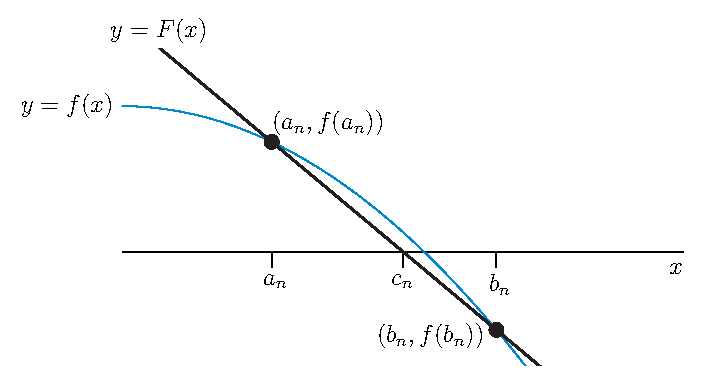
\includegraphics{falsePosition}
\end{center}
\end{efig}
The equation of that straight line is
\begin{equation*}
y = F(x) = f(a_n) + \frac{f(b_n)-f(a_n)}{b_n-a_n}(x-a_n)
\end{equation*}
Then the false position method tests the sign of $f(x)$ at the value of 
$x$ where $F(x)=0$.
\begin{align*}
&F(x) = f(a_n) + \frac{f(b_n)-f(a_n)}{b_n-a_n}(x-a_n)
  =0 \\
& \iff x= a_n - \frac{b_n-a_n}{f(b_n)-f(a_n)} f(a_n)
           = \frac{a_n f(b_n) - b_n f(a_n) }{f(b_n)-f(a_n)}
\end{align*}
So once we have the interval $I_n$, the false position method generates the interval $I_{n+1}$ by the following rule.\footnote{The convergence behaviour of the false position method is relatively complicated. So we do not discuss 
it here. As always, we invite the interested reader to visit their favourite search engine.}
\begin{impeqn}[fale position method]\label{eq:APPfalsePosition}
Set $c_n=\frac{a_n f(b_n) - b_n f(a_n) }{f(b_n)-f(a_n)}$. 
If $f(c_n)$ has the same sign as $f(a_n)$, then
  \begin{equation*}
    I_{n+1}=[a_{n+1},b_{n+1}]\quad\text{with}\quad
               a_{n+1}=c_n,\  b_{n+1}=b_n
  \end{equation*}
and if 
$f(c_n)$ and $f(a_n)$ have opposite signs, then
  \begin{equation*}
    I_{n+1}=[a_{n+1},b_{n+1}]\quad\text{with}\quad
             a_{n+1}=a_n,\  b_{n+1}=c_n
  \end{equation*}
\end{impeqn}


\begin{comment}
As an example, we repeat Example \ref{eg bisection}, but using the false position 
method in place of the bisection method. 
\begin{eg}[Exmple \ref{eg bisection}, continued]\label{eg false position}
In Example \ref{eg bisection} we used the bisection method to look a zero of
\begin{align*}
  f(x) &= x-1+\sin(\pi x/2)
\end{align*}
that lies between $0$ and $1$. In this example we use the false position method instead.

We start with
\begin{itemize}
 \item $a_1=0,$ $b_1=1$ and
  $f(a_1) = -1$,
  $f(b_1) = 1$.
 \item Test the point 
\begin{equation*}
 x = c_1 = \frac{a_1 f(b_1) - b_1 f(a_1) }{f(b_1)-f(a_1)}
         = \frac{0 (1) -(1)(-1) }{(1)-(-1)} = 0.5
\end{equation*}
which, in this special case, happens to be the midpoint of $I_1$.
\begin{align*}
  f(0.5) &= 0.2071067813 > 0
\end{align*}
\item So our new interval will be $[0,0.5]$ since the function is negative at
$x=0$ and positive at $x=0.5$
\end{itemize}
Repeat
\begin{itemize}
 \item $a_2=0, b_2=0.5$ where $f(a_2)=-1<0$ and $f(0.5)=0.2071067813>0$.
 \item Test the point 
\begin{equation*}
 x = c_2 = \frac{a_2 f(b_2) - b_2 f(a_2) }{f(b_2)-f(a_2)}
         = 0.4142135624
\end{equation*}
\begin{align*}
  f(0.4142135624) &= 0.1991242945 > 0
\end{align*}
\item So our new interval will be $[0,0.4142135624]$ since the function 
is negative at $x=0.0$ and positive at $x=0.4142135624$
\end{itemize}
\end{eg}
\end{comment}
%%%%%%%%%%%%%%%%%%%%%%%%%%%%%%%%%%%%%%%%%%%%%%%%%%%%%%%%%%%%%%%
\section{The secant method}\label{sec_C_4}
%%%%%%%%%%%%%%%%%%%%%%%%%%%%%%%%%%%%%%%%%%%%%%%%%%%%%%%%%%%%%%%%
Let $f(x)$ be a continuous function. The secant method is a variant of 
Newton's method that avoids the use of the derivative of $f(x)$ --- which can be very helpful when dealing with the derivative is not easy. It avoids the use of the derivative  by approximating  $f'(x)$ by $\frac{f(x+h)-f(x)}{h}$ for some $h$. That is, it approximates the tangent line to $f$ at $x$ by a secant line 
to $f$ that passes through $x$. To limit the number of evaluations of $f(x)$ required, it uses $x=x_{n-1}$ and $x+h=x_n$. Here is how it works.

Suppose that we have already found $x_n$. Then we denote by $y=F(x)$ the equation of the (secant) line that passes through 
$\big(x_{n-1}, f(x_{n-1})\big)$  and $\big(x_n,f(x_n)\big)$ and we choose $x_{n+1}$ to be the value of $x$ where $F(x)=0$. 
\begin{efig}
\begin{center}
   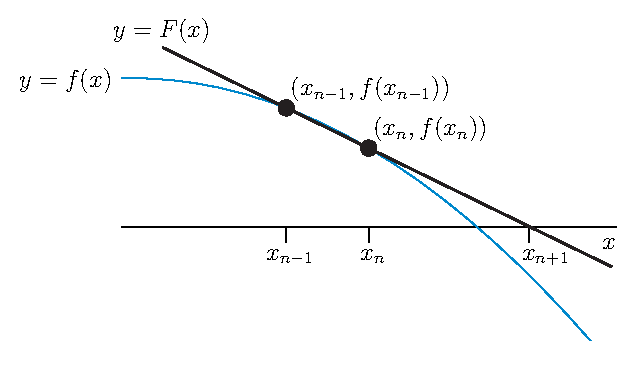
\includegraphics{secant}
\end{center}
\end{efig}
The equation of the secant line is
\begin{equation*}
y = F(x) = f(x_{n-1}) + \frac{f(x_n)-f(x_{n-1})}{x_n-x_{n-1}}(x-x_{n-1})
\end{equation*}
so that $x_{n+1}$ is determined by
\begin{align*}
&0=F(x_{n+1}) = f(x_{n-1}) + 
    \frac{f(x_n)-f(x_{n-1})}{x_n-x_{n-1}}(x_{n+1}-x_{n-1})
 \\
& \iff x_{n+1}= x_{n-1} - \frac{x_n-x_{n-1}}{f(x_n)-f(x_{n-1})} f(x_{n-1})
%           = \frac{x_{n-1} f(x_n) - x_n f(x_{n-1}) }{f(x_n)-f(x_{n-1})}
\end{align*}
or, simplifying,
\begin{impeqn}[secant method]\label{eq:APPsecant}
  \begin{equation*}
    x_{n+1}=\frac{x_{n-1} f(x_n) - x_n f(x_{n-1}) }{f(x_n)-f(x_{n-1})}
  \end{equation*}
\end{impeqn}
Of course, to get started with $n=1$, we need two initial guesses, $x_0$ and $x_1$, for the root.

\begin{eg}[Approximating $\sqrt{2}$, again]\label{eg:NTMsqrttwoC}
In this example we compute, approximately, the square root of two by
applying the secant method to the equation
\begin{equation*}
f(x)=x^2-2=0
\end{equation*}
and we'll compare the secant method results with the corresponding Newton's method results.
(See Example \ref{eg:NTMsqrttwo}.)

Since $f'(x)=2x$, \eqref{eq:APPnewton} says that, under Newton's method, 
we should iteratively apply
\begin{equation*}
x_{n+1}=x_n-\frac{f(x_n)}{f'(x_n)}=x_n-\frac{x_n^2-2}{2x_n}
=\frac{x_n}{2} +\frac{1}{x_n}
\end{equation*}
while \eqref{eq:APPsecant} says that, under the secant method, 
we should iteratively apply (after a little simplifying algebra)
\begin{align*}
x_{n+1}&=\frac{x_{n-1} f(x_n) - x_n f(x_{n-1}) }{f(x_n)-f(x_{n-1})}
       =\frac{x_{n-1}[x_n^2-2] - x_n[x_{n-1}^2-2] }{x_n^2-x_{n-1}^2} \\
       &=\frac{x_{n-1}x_n[x_n-x_{n-1}]+2[x_n-x_{n-1}]}{x_n^2-x_{n-1}^2} \\
       &=\frac{x_{n-1}x_n+2}{x_{n-1}+x_n}
\end{align*}
Here are the results, starting Newton's method with $x_1=4$ and starting
the secant method with $x_0=4$, $x_1=3$. (So we are giving the secant method 
a bit of a head start.)
\begin{alignat*}{5}
&  &&\text{secant method}\qquad &&\text{Newton's method} \\
&x_0\quad && 4 && \\
&x_1 && 3 && 4 \\
&x_2 && 2 && 2.25 \\
&x_3 && 1.6 && 1.57 \\
&x_4 && 1.444 && 1.422 \\
&x_5 && 1.4161 && 1.414234 \\
&x_6 && 1.414233 && 1.414213562525 \\
&x_7 && 1.414213575 && 1.414213562373095
\end{alignat*}
For comparison purposes, the square root of $2$, to 15 decimal places,
is $1.414213562373095$. %%% 1.4142135623730950488
So the secant method $x_7$ is accurate to 7 decimal places 
and the Newton's method $x_7$ is accurate to at least 15 decimal places.



\end{eg}


 
The advantage that the secant method has over Newton's method is that it does not use the derivative of $f$. This can be a substantial advantage, for example  
when  evaluation of the derivative is computationally difficult or expensive. 
On the other hand, the above example suggests that the secant method is not 
as fast as Newton's method. The following section shows that this is indeed the case.

\section{The Error Behaviour of the Secant Method}\label{sec_C_5}

Let $f(x)$ have two continuous derivatives, and let $r$ be any solution 
of $f(x)=0$. 
We will now get a pretty good handle on the error behaviour of the secant method 
near $r$.

Denote by $\tilde\veps_n=x_n-r$ the (signed) error in $x_n$ and by
$\veps_n=|x_n-r|$ the (absolute) error in $x_n$. Then, 
$x_n =r+\tilde\veps_n$, and, by \eqref{eq:APPsecant}, 
\begin{align*}
\tilde\veps_{n+1} 
         &= \frac{x_{n-1} f(x_n) - x_n f(x_{n-1}) }{f(x_n)-f(x_{n-1})} -r \\
         &= \frac{[r+\tilde\veps_{n-1}] f(x_n) - [r+\tilde\veps_n] f(x_{n-1}) }
                                            {f(x_n)-f(x_{n-1})} -r \\
         &= \frac{\tilde\veps_{n-1} f(x_n) - \tilde\veps_n f(x_{n-1}) }
                                            {f(x_n)-f(x_{n-1})}
\end{align*}


By the Taylor expansion \eqref{eq:taylorErrorQ}
and the mean value theorem (Theorem \ref{thm:DIFFmvt}),
\begin{align*}
f(x_n)&= f(r) + f'(r)\tilde\veps_n +\frac{1}{2} f''(c_1) \tilde\veps_n^2 \\
      &= f'(r)\tilde\veps_n +\frac{1}{2} f''(c_1) \tilde\veps_n^2 \\
f(x_n)-f(x_{n-1})&= f'(c_2)[x_n-x_{n-1}] \\
                &= f'(c_2)[\tilde\veps_n-\tilde\veps_{n-1}]
\end{align*}
for some $c_1$ between $r$ and $x_n$ and some $c_2$ between $x_{n-1}$ and $x_n$. 
So, for $x_{n-1}$ and $x_n$ near $r$, $c_1$ and $c_2$ also have to be near $r$ and
\begin{align*}
f(x_n)&\approx f'(r)\tilde\veps_n +\frac{1}{2} f''(r) \tilde\veps_n^2 \\
f(x_{n-1})&\approx f'(r)\tilde\veps_{n-1} +\frac{1}{2} f''(r) \tilde\veps_{n-1}^2 \\
f(x_n)-f(x_{n-1})&\approx f'(r)[\tilde\veps_n-\tilde\veps_{n-1}] 
\end{align*}
and
\begin{align*}
\tilde\veps_{n+1} &= \frac{\tilde\veps_{n-1} f(x_n) - \tilde\veps_n f(x_{n-1}) }
                                              {f(x_n)-f(x_{n-1})} \\
 &\approx \frac{ \tilde\veps_{n-1} [f'(r)\tilde\veps_n +\frac{1}{2} f''(r) \tilde\veps_n^2]
               -  \tilde\veps_n [f'(r)\tilde\veps_{n-1} +\frac{1}{2} f''(r) \tilde\veps_{n-1}^2] }
                    { f'(r)[\tilde\veps_n-\tilde\veps_{n-1}] }  
\\
  &= \frac{\frac{1}{2}\tilde\veps_{n-1}\tilde\veps_nf''(r)[\tilde\veps_n-\tilde\veps_{n-1}]}
               { f'(r)[\tilde\veps_n-\tilde\veps_{n-1}] } 
\\
&= \frac{f''(r)} {2f'(r)} \tilde\veps_{n-1}\tilde\veps_n
\end{align*}
Taking absolute values, we have
\begin{equation*}
\veps_{n+1}\approx K \veps_{n-1}\veps_n\qquad
\text{with }K = \left|\frac{f''(r)} {2f'(r)} \right|
\tag{E7}\end{equation*} 
We have seen that Newton's method obeys a similar formula ---
(E3) says that, when $x_n$ is near $r$, Newton's method obeys $\veps_{n+1}\approx K\veps_n^2$, also with 
$K = \left|\frac{f''(r)} {2f'(r)} \right|$.
As we shall now see, the change from $\veps_n^2$, in 
$\veps_{n+1}\approx K\veps_n^2$, to $\veps_{n-1}\veps_n$, in 
$\veps_{n+1}\approx K\veps_{n-1}\veps_n$,
does have a substantial impact on the behaviour of $\veps_n$ for large $n$.

To see the large $n$ behaviour, we now iterate (E7). The formulae will look simpler if we multiply (E7) by $K$ and write $\delta_n=K\veps_n$.
Then (E7) becomes $\delta_{n+1}\approx\delta_{n-1}\delta_n$ (and we have eliminated $K$). 
The first iterations are
\begin{alignat*}{3}
\delta_2&& &\approx \delta_0\delta_1 \\
\delta_3&\approx \delta_1\delta_2 
       &&\approx \delta_0\delta_1^2 \\
\delta_4&\approx \delta_2\delta_3 
       &&\approx \delta_0^2\delta_1^3 \\
\delta_5&\approx \delta_3\delta_4 
       &&\approx \delta_0^3\delta_1^5 \\
\delta_6&\approx \delta_4\delta_5 
       &&\approx \delta_0^5\delta_1^8 \\
\delta_7&\approx \delta_5\delta_6 
       &&\approx \delta_0^8\delta_1^{13}
\end{alignat*}
Notice that every $\delta_n$ is of the form 
                $\delta_0^{\alpha_n}\delta_1^{\beta_n}$.
Substituting $\delta_n=\delta_0^{\alpha_n}\delta_1^{\beta_n}$ into $\delta_{n+1}\approx\delta_{n-1}\delta_n$ gives
\begin{equation*}
\delta_0^{\alpha_{n+1}}\delta_1^{\beta_{n+1}} 
           \approx \delta_0^{\alpha_{n-1}}\delta_1^{\beta_{n-1}}
                               \delta_0^{\alpha_n}\delta_1^{\beta_n}
\end{equation*}
and we have
\begin{equation*}
\alpha_{n+1}=\alpha_{n-1}+\alpha_{n} \qquad
\beta_{n+1}=\beta_{n-1}+\beta_{n} 
\tag{E8}\end{equation*}

The recursion rule in (E8) is famous\footnote{Plug ``Fibonacci sequence in nature'' into your search engine of choice.}. The 
Fibonacci\footnote{Fibonacci (1170-1250) was an Italian mathematician who was also known as Leonardo of Pisa, Leonardo Bonacci and Leonardo Biglio Pisano.} 
sequence (which is $0$, $1$, $1$, $2$, $3$, $5$, $8$, $13$, $\cdots$), 
is defined by 
\begin{align*}
F_0&=0 \\ 
F_1&=1 \\ 
F_n&=F_{n-1}+F_{n-2}\qquad\text{for }n>1
\end{align*}
So, for $n\ge 2$, $\alpha_n = F_{n-1}$ and $\beta_n=F_n$ and
\begin{equation*}
\delta_n \approx \delta_0^{\alpha_n}\delta_1^{\beta_n}
         = \delta_0^{F_{n-1}}\delta_1^{F_n}
\end{equation*}
One of the known properties of the Fibonacci sequence is that, for large $n$,
\begin{equation*}
F_n\approx\frac{\varphi^n}{\sqrt{5}}\qquad\text{where }
\varphi=\frac{1+\sqrt{5}}{2} \approx 1.61803 
\end{equation*}
This $\varphi$ is the golden ratio\footnote{Also worth a quick trip to your search engine.}. 
So, for large $n$,
\begin{align*}
K\veps_n &= \delta_n
         \approx \delta_0^{F_{n-1}}\delta_1^{F_n}
         \approx \delta_0^{\frac{\varphi^{n-1}}{\sqrt{5}}}
                               \delta_1^{\frac{\varphi^n}{\sqrt{5}}}
         = \delta_0^{\frac{1}{\sqrt{5}\varphi}\times\varphi^n}
                          \delta_1^{\frac{1}{\sqrt{5}}\times\varphi^n}
\\
&= d^{\varphi^n}\qquad\text{where}\quad
   d=\delta_0^{\frac{1}{\sqrt{5}\,\varphi}}\delta_1^{\frac{1}{\sqrt{5}}}
\\
&\approx d^{1.6^n}
\end{align*}
Assuming that $0<\delta_0=K\veps_0<1$ and $0<\delta_1=K\veps_1<1$,
we will have $0<d<1$. 

By way of contrast, for Newton's method, for large $n$,
\begin{align*}
K\veps_n\approx d^{2^n}\qquad\text{where}\quad
                d=(K\veps_1)^{1/2}
\end{align*}
As $2^n$ grows quite a bit more quickly than $1.6^n$ 
(for example, 
        when n=5, $2^n=32$ and $1.6^n=10.5$, 
    and when $n=10$, $2^n=1024$ and $1.6^n=110$)
Newton's method homes in on the root quite a bit faster than the secant method,
assuming that you start reasonably close to the root.
